\chapter{模式构架}\label{模式构架}
%\addcontentsline{toc}{chapter}{模式结构}
\section{网格构建}\label{网格构建}

通用陆面模式(CoLM,Common Land Model)首先对陆地表面进行剖分,将模拟区域按一定规则划分成单元(Element),模拟分辨率决定了单元平均面积的大小。CoLM中包含三种单元划分规则:1)经纬度网格;2)非结构网格(三角形/六边形);3)流域单元(Catchment)。

经纬度网格通过规定经度和纬度分割线的位置来建立,单元的边界由东西两段经线和南北两段纬线组成。经纬度网格的分辨率通常使用经纬度分割线的间距来表达,例如,分辨率为0.5\textdegree 表示相邻两条纬度分割线和经度分割线的距离均为0.5\textdegree。


包括三角形网格和六边形网格在内的非结构网格是一种无规则拓扑关系的网格。与经纬度网格相比,非结构网格的分辨率取决于指定一个或者多个目标的分布特征(例如高程、坡度、土地利用、植被类型等),在目标变化梯度较大的地区采用高分辨率,而在变化梯度较小的地区采用低分辨率。因此非结构化基于网格的多分辨率模拟保留了全局模型的整体结构,同时支持局部区域的高分辨率模拟。非结构网格的构建是基于 Delaunay 三角网等值线生成算法,首先将经纬度网格数据转化插值,生成铺盖整个球面的三角形网格数据;接着根据所选取的目标进行一次或者多次细化;再通过连接具有相同顶点的六个三角形三条边的重心生成蜂窝六边形(使用六边形网格的情况下),最后生成全球或者区域的三角形或六边形可变分辨率网格。

流域单元网格通过对河网进行分段来建立,一个单元定义为一段河道的集水区域,流域单元之间具有明确的上下游关系。流域单元网格的分辨率使用单元的面积阈值(即河道集水区域的面积阈值)来表达,自然连通的湖泊设置为独立的单元,不受面积阈值的限制。
\subsection{经纬度网格}\label{经纬度网格}

\subsection{流域单元网格}\label{流域单元网格}

\subsection{非结构网格}\label{非结构网格}
非结构网格是一种无规则拓扑关系的网格,通常由各种不规则多边形组成。与结构(方形)网格相比,非结构网格的分辨率取决于指定目标的分布特征[]。非结构化基于网格的多分辨率模拟保留了全局模型的整体结构,同时支持局部区域的高分辨率模拟。与结构网格相比,非结构网格具有灵活性强、节点和单元的分布可控性好、能较好地控制网格的大小和节点的密度的优点,并且它弥补了结构网格不能够解决任意形状和连通区域的网格剖分的缺陷。

在原有的经纬度网格的基础上,CoLM新开发了一个非结构化网格构建工具,可以基于多目标(水平分布特征),如高程、坡度、地形、土地利用和植被类型,自动识别不同区域所需的网格分辨率。模式运行流程如图~\ref{fig:非结构化网格CoLM总体运行流程图} 所示:
 {
\begin{figure}[]
\centering
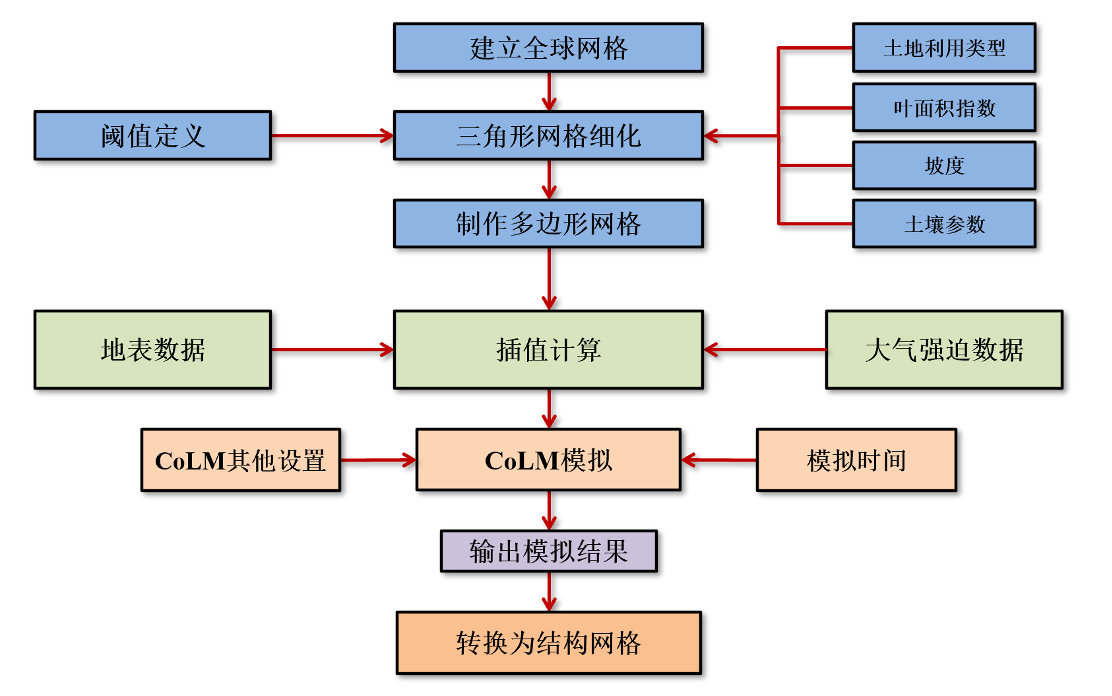
\includegraphics{Figures/模式构架/非结构化网格CoLM总体运行流程图.png}
\caption{非结构化网格CoLM总体运行流程图,摘自Fan et al. [2023, in preparation]。}
\label{fig:非结构化网格CoLM总体运行流程图}
\end{figure}
}

该工具基于非结构化一致性三角-六边形构建算法 \citep{fatichi2020soil,walko2008ocean,walko_direct_2011},以准均匀的全局三角形(Delaunay)的网格化方法为理论依据。在CoLM中的非结构网格运行流程如图~\ref{fig:非结构化网格生成流程图} 所示,具体介绍如下:
{
\begin{figure}[]
\centering
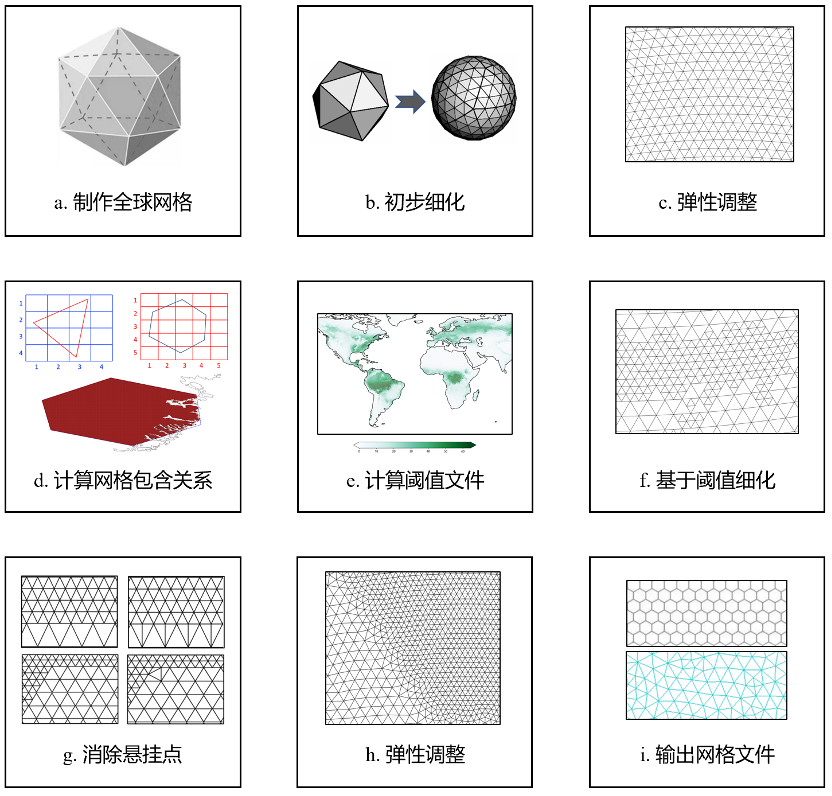
\includegraphics{Figures/模式构架/非结构化网格生成流程图.png}
\caption{非结构化网格生成流程图,摘自Fan et al. [2023, in preparation]。}
\label{fig:非结构化网格生成流程图}
\end{figure}
}

{
\begin{table}[]
\centering
\caption{细化阈值文件}
\label{tab:细化阈值文件}
\begin{tabular}{@{}ll@{}}
\toprule
变量名            & 具体描述           \\\midrule
num\_landtypes & 网格包含的土地类型数量    \\
f\_mainland    & 网格主导土地类型       \\
max\_iter      & 三角形网格最大细化迭代次数  \\
lai            & 叶面积指数          \\
slope          & 坡度             \\
k\_s           & 饱和导水率          \\
k\_solids      & 土壤固体导热系数       \\
tkdry          & 土壤导热系数(干燥)     \\
tksatf         & 土壤导热系数(冻结、饱和)  \\
tksatu         & 土壤导热系数(未冻结、饱和) \\\bottomrule
\end{tabular}
\end{table}
}

 {
\begin{figure}[]
\centering
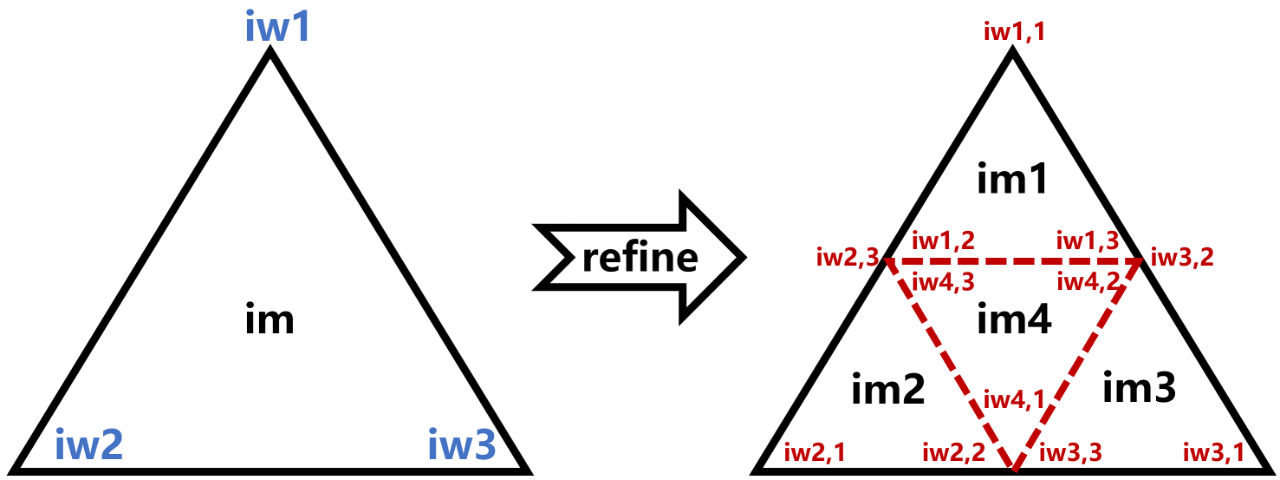
\includegraphics{Figures/模式构架/三角形网格简易细化.png}
\caption{三角形网格简易细化,摘自Fan et al. [2023, in preparation]}
\label{fig:三角形网格简易细化}
\end{figure}
}

\begin{enumerate}
\item 构建初始网格\\
在此过程中,首先将一个正二十面体投射到地球表面,它的12个顶点中有两个位于南北两极,其余的位于$\pm\arctan(1/2)$ 纬度。构建好的正二十面体网格的二维投影在0\textdegree 经线与0\textdegree 纬线是轴对称的,有利于在计算包含关系时简化运算步骤。同时将每个区域划分为面积相同大小的三角形分块,以满足非结构网格初步细化和提升并行化计算效率的需要。
\item 初步细化\\
在此步骤中,网格生成工具能够将每个球面三角形面细分为NXP×NXP更小的三角形,其中NXP是可以设置为任意正整数,代表所选的网格分辨率。其定义是两个相邻六边形网格的水平网格间距(网格单元面积的平方根)。网格的分辨率大约等于7200公里/NXP。因此,如果试图在网格上获得100公里的水平网格间距,则应将NXP设置为“72”。这种网格配置采用基于二十面体改进的六边形或三角形网格单元的非结构化网格,从而避免了传统经纬度网格的南北极奇点。该网格配置为局部网格细化提供了一种完全无缝的自然适应性,不需要额外特殊的网格嵌套算法。
\item 弹簧动态调整\\
虽然通过初步的细化生成的三角形在平面上看起来是等边三角形,但实际上并不完全等同于等边三角形,有一定的角度偏差。实际上,如果考虑到经纬度基础数据在高纬度形变的影响,三角形的变形也会随着纬度的增加而增加。\citet{tomita2002optimization}描述了一种称为“Spring Dynamics”的计算方法,用于在准均匀的全局网格上调整三角形网格单元的形状和大小。该方法代表了一种物理模拟,其中网格中的每个边都像弹簧一样在其端点(顶点)之间施加吸引力或相反的力,该弹力取决于其自身的长度、平衡长度和弹簧系数。该研究表明,将平衡长度设置为使弹簧松弛在数值上稳定的最大可能值,即接近整个网格的平均边长,会产生最小的网格单元尺寸的空间变化,并且调整过程能显著提高模型的数值精度。
\item 计算包含关系 \\
CoLM非结构网格的空间细分基于三角形网格与阈值数据(部分地表数据,如表~\ref{tab:细化阈值文件})进行。一般来说,三角形网格的分辨率远高于阈值数据集。这些高分辨率网格(以下简称像素)构成了非结构化网格。也就是说,每个非结构化网格包含多个高分辨率像素。在进行网格细化之前,需要得到每个网格对应的像素的索引,即计算包含关系,以便识别像素对非结构网格的归属。最后,根据这些像素的信息,用户可以了解特定网格内的空间异质性,并决定是否需要对其进行细化。这个过程将在细化过程中的每次迭代中执行。
\item 阈值文件计算\\
最初,\citet{walko_direct_2011} 中的细化面积和程度是通过分配一系列点的经纬度坐标来确定的(例如,(lat = 30.1, lon = 120.5); \dots)加上影响半径(例如,(R = 1km); \dots)。与之不同,CoLM的网格细化工具能够根据各种指标确定精细化的区域。关于这些指标的详细信息可以在表~\ref{tab:细化阈值文件} 中找到。该工具允许对一个或多个对象的网格细化约束到用户定义的阈值。也就是说,CoLM可以根据任意数量的重要特征对网格进行细化,例如$LAI$的标准差,网格内土地利用类型数量等等。图~\ref{fig:多阈值非结构网格细化} 展示了基于多种不同地表特征进行细化的所生成的全球六边形网格结构。
 {
\begin{figure}[]
\centering
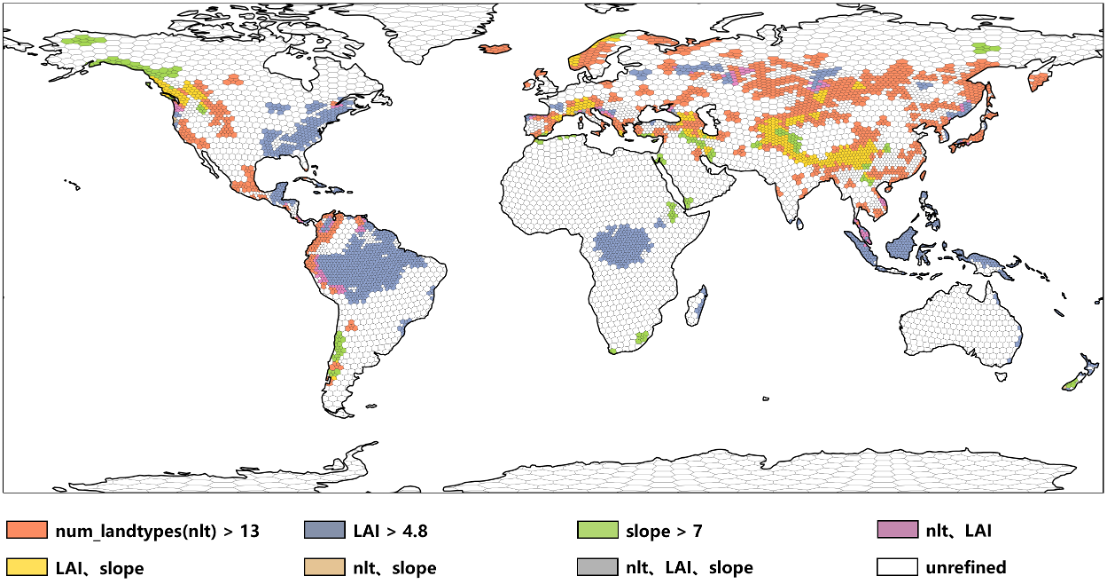
\includegraphics{Figures/模式构架/多阈值非结构网格细化.png}
\caption{多阈值非结构网格细化示例,摘自Fan et al. [2023, in preparation]}
\label{fig:多阈值非结构网格细化}
\end{figure}
}

\item 阈值细化\\
如图~\ref{fig:非结构化网格生成流程图} 所示,本步骤主要实现三角网格的阈值细化。利用生成的初始三角网格包含关系,计算三角网格下各阈值类型的数组,然后根据阈值标记网格是否需要细化。如图~\ref{fig:三角形网格简易细化} 所示,通过将三角网格“分成四格”,提高了三角网格的分辨率。然后,将新生成的网格信息添加到原始数组中,并添加精细的网格标记。在计算更新网格的包含关系时,只需要遍历精化三角形最小外围矩形内的经纬度网格,可以大大减少计算时间。当迭代次数超过最大迭代阈值,或所有三角形网格满足阈值时,三角形非结构化网格阈值细化终止。程序将输出最终生成的带有包含信息的三角网格信息数据(见表~\ref{tab:细化阈值文件})。图~\ref{fig:根据LAI对非结构网格进行多重细化} 展示了基于叶面积指数特征不同细化的区域六边形网格结构。
 {
\begin{figure}[]
\centering
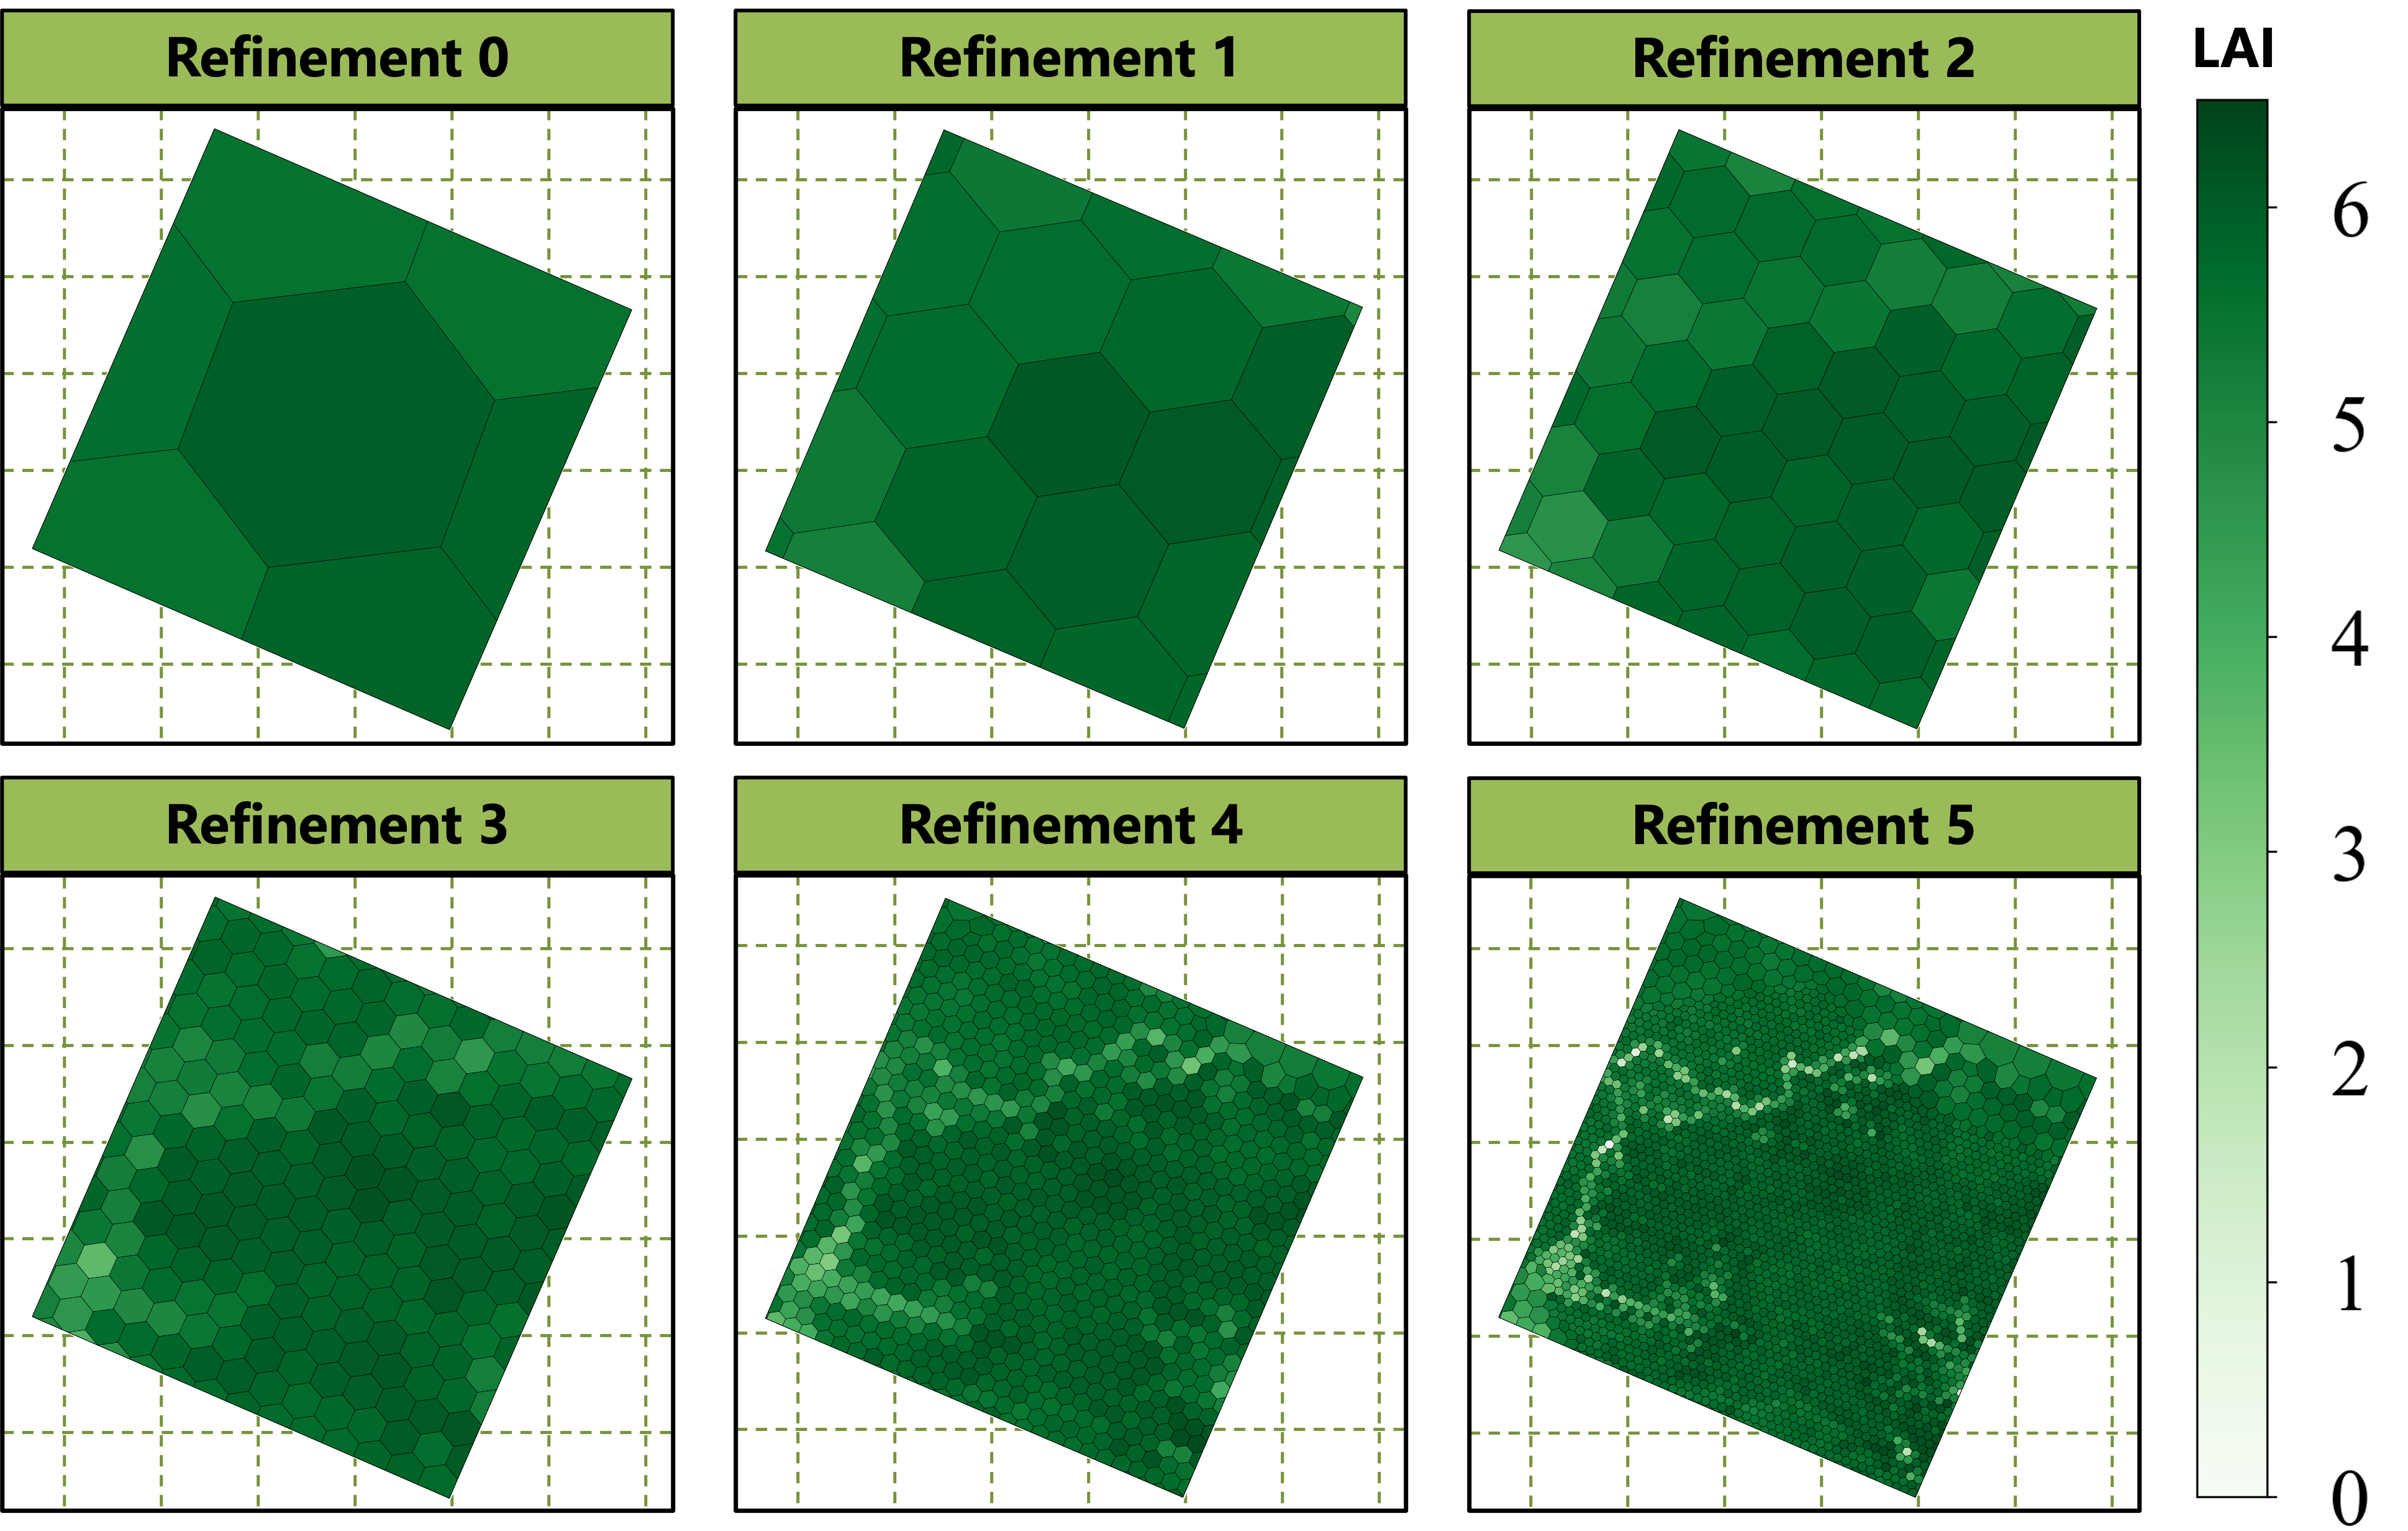
\includegraphics{Figures/模式构架/根据LAI对非结构网格进行多重细化.png}
\caption{根据LAI对非结构网格进行多重细化,摘自Fan et al. [2023, in preparation]}
\label{fig:根据LAI对非结构网格进行多重细化}
\end{figure}
}


\item 清除悬挂点\\
我们把网格细化生成的附着在原始三角形边缘上的点称为悬挂点。对于悬挂点,我们针对两种情况选择了两种不同的消除方法。如图~\ref{fig:非结构化网格生成流程图} 顶部所示,对于细化边缘较平坦的区域,可以连接悬挂点与其相邻三角形的顶点。然而,对于一些凹陷区域,如图~\ref{fig:非结构化网格生成流程图} 底部所示,悬挂点处于相邻位置。直接连接悬挂点与其相邻三角形的顶点会使顶点被相邻的8条边共享,在生成多边形网格时产生八边形网格。因此,如图~\ref{fig:非结构化网格生成流程图} 底部所示,我们采用了特殊的细化方法来避免这一问题。

此外,在消除挂节点时,如果两个细化区域的边界相遇,则容易产生7个以上三角形网格顶点的相邻边。因此,在消除挂节点之前,需要对初步细化后的网格进行如下预处理:
\begin{enumerate}
\item 遍历所有未细化的三角网格。当其相邻的3个三角形网格中有1个以上被细化时,该三角形网格需要被细化。
\item 在三角形网格中找到并记录凹陷区域(即图~\ref{fig:非结构化网格生成流程图} 底部细化区域)。当两个凹陷区域有一个公共三角形网格时,细化组成它们的三个三角形网格。
\item 循环遍历所有三角形网格顶点,计算剔除悬挂节点后该点将添加的邻接边数,当增加后邻接边数大于7时,细化该点的所有邻接三角形网格。
在预处理过程中,三个进程依次进入迭代。当三个过程同时没有添加新的细化网格时,视为预处理完成。预处理后,可以进行消除挂节点的操作(即图~\ref{fig:非结构化网格生成流程图}),得到可以用多边形网格构建的三角形网格。
\end{enumerate}
\item 网格调整和多边形网格生成\\
三角形网格构造完成后,消除凹陷区域后会生成许多钝角三角形,而多边形网格是由三角形网格重心连接而成的。因此,这会导致在多边形网格的生成过程中,一些多边形与正多边形偏差较大,降低了网格的各向同性,从而影响了网格在CoLM等水文模型中的应用。为了在不过度影响原有网格结构的情况下对网格进行校正。
\item 输出网格文件\\
在上述步骤完成之后,可以输出两种类型的网格。第一种一是最后一次迭代生成的三角形网格,第二种是根据三角形网格重心连接的六边形网格。在MPI版本中,无需将地表、大气等初始数据的存储方式由经纬度网格转换为非结构化网格,就可以实现CoLM中地表水文过程在非结构化网格上的模拟。
\end{enumerate}

更为详细的网格制作过程参考附录。


\section{次网格结构}\label{次网格}

考虑到地表下垫面覆盖的异质性,CoLM对模式网格单元进一步划分次网格。
次网格是CoLM计算模拟的基本结构单元,通常称为patch(斑块)。
Patch是通过使用高分辨率的精细化网格数据,根据网格单元内部地表覆盖类型、植被功能类型、叶面积指数、土壤属性和地形等分布特征,按一定方式进行划分并聚合而来。Patch是用于模拟网格单元内部不同下垫面覆盖过程(对地表异质性考虑),同时也起到了减少计算量作用。


由patch可以组成按经纬度网格(章节~\ref{经纬度网格})、流域单元网格(章节~\ref{流域单元网格})及非结构(章节~\ref{非结构网格})网格。
在patch尺度计算得到的通量按其所在网格覆盖比例进行面积加权平均,作为地表网格通量模拟结果。
地表状态或预报变量一般情况下亦是如此,在patch尺度计算得到的结果按照面积加权平均后作为模式结果输出。


CoLM patch从大类上分为五类:植被(含裸土)、城市、湿地、冰川和水体,另外加上海洋。其中植被和城市patch可根据不同类型进一步细分。


植被patch可以分为自然植被和作物。自然植被patch采用三种次网格植被结构进行表征:1) 地表覆盖类型--LCT (Land Cover Type);2) 植被功能型--PFT (Plant Function Type)和3) 植物群落--PC (Plant Community)。以上三种方式,模式运行时只能选择其中一种。
LCT方案为CoLM2014版原有方案,即将某一地表覆盖类型可能包含的多种功能型植被当成混合植被进行模拟,其设置的相关参数可视为等效参数。例如热带大草原,虽然可能包含树和草,但仍视为一种植被,因此相应的植被参数只有一套。
PFT是目前陆面模式(如CLM和JULES)常采用的次网格表征方式,也是本版本CoLM新添加的方式。
PFT方案是将每一个细网格地表覆盖类型进行拆解,得到其PFT的组成种类和各自面积占比,并将其聚合到模式网格中。
本版本CoLM PFT方案类似于CLM PFT方案,即模式格点中的所有PFT作为1个植被patch,共享土壤水热等环境,但各PFT的辐射和通量等过程计算相对独立。
PC方案保留LCT方案中模拟对象,即地表覆盖类型,同时还进一步对LCT中的地表覆盖植被类型进行PFT细分。
不同于LCT方案把某一类型地表覆盖的所有植被视为混合植被,PC方案对某一地表覆盖类型所组成的PFT进行显式表达计算,所有PFT在同一地表覆盖类型中共享土壤水热等环境,同时辐射和通量计算等过程相互影响、同时求解,即考虑了PFT之间的共存与竞争。这一方案类似于植物群落的概念,故命名为PC (Plant Community)方案。


LCT方案所依赖的地表覆盖类型数据可以直接由USGS (章节~\ref{USGS地表覆盖数据})或者MODIS-IGBP地表覆盖数据获取(章节~\ref{IGBP地表覆盖数据})。PFT和PC方案所需要的植被结构及属性数据由MODIS-IGBP地表覆盖数据加以其他辅助数据制作而成(章节~\ref{PFTPC数据及其依赖数据})。


对于作物patch,当作物模式未打开时,作物被当成一种特殊的自然植被进行模拟;当打开作物模式时,
每个模式格点根据包含的作物分类及组成比例(外部数据读取)分别建立相互独立的patch进行模拟计算,方式同PFT方案。
城市patch与作物类似,当城市模式未打开时,城市被当成一种地表覆盖进行模拟,即薄板城市模型(Slab Urban);
当城市模式打开时,每个模式格点根据包含的城市类型和组成比例(根据几何参数)分别建立相互独立的patch进行模拟计算。
目前城市分类提供两种方式:
\begin{enumerate}
    \item 根据城市密度分为高建筑、高密度和中密度3类(基于NCAR CLMU城市模式);
    \item 根据城市局地气候区(LCZ,Local Climate Zone)分为10类。
\end{enumerate}
城市分类及其属性数据从外部数据读取(章节~\ref{城市数据})。

\section{计算框架}\label{计算框架}



\section{陆气耦合}\label{陆气耦合}
\subsection{陆面模式与大气模式的数据交换}
陆面模式的运行需要当前时刻的大气状态作为驱动。当陆面模式离线运行时(offline),大气状态可由观测数据、再分析数据或大气模式模拟结果数据直接提供;当陆面模式置于天气/气候/地球系统模式耦合运行时(online),大气状态可由大气模式通过耦合器或程序调用接口实时传递给陆面模式。陆面模式接收到当前时刻的大气状态后,首先结合上一时刻的植被、雪盖或土壤的状态和地表特征(如地表反照率、空气动力学阻抗等)计算当前时刻的陆气湍流交换通量、辐射通量、进入地表的能量和水分通量等,然后基于这些通量条件计算当前时刻的植被、雪盖或土壤的状态变量和地表特征量。在耦合运行时,这些地表通量和状态变量实时返回给大气,为大气模式进行下一时刻的计算提供下边界条件。陆面模式所需的大气变量和大气模式所需的陆面变量详见表~\ref{tab:陆面模式所需的大气状态变量} 和表~\ref{tab:大气模式所需的陆面模式输出变量}。

关于参考高度(reference height) (见表~\ref{tab:陆面模式所需的大气状态变量}),即大气驱动变量所在的高度,需要做一点特殊说明。参考高度的设置通常比较随意,一般认为只要不超过近地层即可。在陆面模式离线运行试验中,参考高度通常为10 m到50 m的高度;在陆气耦合试验中,参考高度通常设为大气模式的最底层。但本团队的最新研究\citep{liu2023referenceheight} 表明,把参考高度设置在近地层顶附近,可以显著提高地表湍流通量的模拟精度。考虑1 km的典型对流边界层高度,建议参考高度设置为100 m左右。

{
\begin{table}[]
\centering
\caption{陆面模式所需的大气状态变量}
\label{tab:陆面模式所需的大气状态变量}
\begin{threeparttable}
\begin{tabular}{lcc}
\toprule
大气状态变量               & 变量名           & 单位           \\  \midrule
大气风速参考高度             & $z_{atm,m}$   & m            \\
大气温度参考高度             & $z_{atm,h}$   & m            \\
大气比湿参考高度             & $z_{atm,w}$   & m            \\
位于$z_{atm,m}$高度的纬向风速 & $u_{atm}$     & \unit{m.s^{-1}}   \\
位于$z_{atm,m}$高度的经向风速 & $v_{atm}$     & \unit{m.s^{-1}}   \\
位于$z_{atm,h}$高度的大气温度 & $T_{atm}$     & K            \\
位于$z_{atm,w}$高度的大气比湿 & $q_{atm}$     & \unit{kg.kg^{-1}} \\
近地面气压                & $P_{atm}$     & Pa           \\
近地面下行长波辐射            & $L\downarrow$ & \unit{W.m^{-2}}   \\
近地面下行短波辐射            & $S\downarrow$ & \unit{W.m^{-2}}   \\
降水                   & $p$           & \unit{mm.s^{-1}}      \\
二氧化碳浓度               & $c_a$         & ppmv         \\
臭氧浓度                 & $c_o$         & \unit{mol.mol^{-1}}  \\
大气气溶胶沉降速率        & $D_{sp}$      & \unit{kg.m^{-2}.s^{-1}}  \\
氮沉降速率                & $N_{dep}$     & \unit{g(N).m^{-2}.yr^{-1}}   \\
闪电频率                 & $I_l$         & \unit{flash.km^{-2}.hr^{-1}} \\ \bottomrule    
\end{tabular}
\begin{tablenotes}
\footnotesize
\item[1] 根据气溶胶种类和亲水性,气溶胶沉降速率可按照14种不同的气溶胶给出,其中沙尘气溶胶可分为8种(视为4种不同气溶胶颗粒大小的干气溶胶或湿气溶胶),黑碳气溶胶分为3种(干亲水性气溶胶、湿亲水性气溶胶、干疏水性气溶胶),有机碳气溶胶分为3种(干亲水性气溶胶、湿亲水性气溶胶、干疏水性气溶胶)。气溶胶沉降主要用于积雪、冰盖和气溶胶辐射模型 (SNICAR),影响积雪反照率和积雪内部辐射传输过程的计算。 
\item[2] 氮沉降速率用于生物地球化学循环模型(BGC),表征无机氮(主要由氮氧化物 $\mathrm{NO_y}$ 和氮氢化物 $\mathrm{NH_x}$ 组成)在陆地表面的沉降通量。
\item[3] 臭氧浓度用于模拟其对气孔导度等植被生理过程的影响,闪电频率用于火灾模式。
\end{tablenotes}
\end{threeparttable}
\end{table}
}
{
\begin{table}[]
\centering
\caption{大气模式所需的陆面模式输出变量}
\label{tab:大气模式所需的陆面模式输出变量}
\begin{threeparttable}
\begin{tabular}{lcc}
\toprule
陆面模式输出变量    & 变量名                            & 单位      \\ \midrule
潜热通量        & $\lambda_vE_p$+$\lambda\ E_g$+ & \unit{W.m^{-2}}    \\
感热通量        & $H_p$+$H_g$                    & \unit{W.m^{-2}}    \\
水汽通量        & $E_p$+$E_g$                    & \unit{mm.s^{-1}}    \\
纬向动量通量      & $\tau_{p,x}$+$\tau_{g,x}$      & \unit{kg.m^{-1}.s^{-2}} \\
经向动量通量      & $\tau_{p,y}$+$\tau_{g,y}$      & \unit{kg.m.s^{-2}} \\
地表出射长波辐射通量  & $L_p\uparrow$+$L_g\uparrow$    & \unit{W.m^{-2}}    \\
直射光可见光波段反照率 & $\alpha_{vis,dir}$             & -       \\
直射光近红外波段反照率 & $\alpha_{nir,dir}$             & -       \\
漫射光可见光波段反照率 & $\alpha_{vis,dif}$             & -       \\
漫射光近红外波段反照率 & $\alpha_{nir,dif}$             & -       \\
地表辐射温度      & $T_{rad}$                      & K       \\
近地面2 m温度     & $T_{2m}$                       & K       \\
近地面2 m比湿     & $q_{2m}$                       & \unit{kg.kg^{-1}}   \\
近地面10 m风速    & $u_{10m}$                      & \unit{m.s^{-1}}     \\
雪水当量        & $W_{sno}$                      & mm      \\
空气动力学阻抗     & $r_{am}$                       & \unit{s.m^{-1}}     \\
摩擦速度        & $u_\ast$                       & \unit{m.s^{-1}}     \\
净生态系统碳交换通量  &   NEE                      & \unit{g.C.m^{-2}.s^{-1}} \\
氧化亚氮浓度      & $\mathrm{N_2O}$               & \unit{g.N.m^{-2}.s^{-1}}\\
\bottomrule         
\end{tabular}
\begin{tablenotes}
\footnotesize
\item[1] 下标 $p$ 和 $g$ 分别代表网格单元内植被覆盖部分和无植被覆盖部分的计算结果
\item[2] $\lambda_v$ 表示蒸发潜热(\unit{J.kg^{-1}}),$\lambda$ 根据地表水份是否冻结取为蒸发潜热 $\lambda_v$ 或升华潜热 $\lambda_s$。
\end{tablenotes}
\end{threeparttable}
\end{table}
}
\subsection{离线运行CoLM可使用的大气驱动数据集}
CoLM支持多套大气驱动数据集的使用,包括全球格点数据和单点数据,可用数据集列表见表~\ref{tab:可用于驱动CoLM离线运行的大气驱动数据集}。用户也可使用其他数据,只需参照任意一种目前支持的数据集制作成对应的数据格式,并参照该数据对应的namelist提供相应的信息即可使用。特别地,当运行区域或单点模式时,大气驱动数据可选择任意一套覆盖该区域或该点的数据,模式可自动从大气驱动数据中提取出该区域或该点的数据信息来驱动CoLM。

%\begin{landscape}
%\begin{longtable}
%\end{longtable}
%\end{landscape}

% Please add the following required packages to your document preamble:
% \usepackage{booktabs}
\begin{landscape}
%\begin{threeparttable}
\begin{center}
\begin{longtable}{p{3cm}p{3cm}p{2cm}<{\centering}p{2cm}<{\centering}p{4cm}<{\centering}p{6cm}<{\centering}}
\caption{可用于驱动 CoLM 离线运行的大气驱动数据集}
\label{tab:可用于驱动CoLM离线运行的大气驱动数据集}
\\
\hline 
\textbf{驱动名} & \textbf{分辨率}& \textbf{时间范围} & \textbf{空间范围} & \textbf{参考文献} & \textbf{附加说明} \\ 
\hline 
\endfirsthead

\multicolumn{6}{c}%
{{\bfseries \tablename\ \thetable{} -- \kaishu 续表}} \\
\hline
\textbf{驱动名} & \textbf{分辨率} & \textbf{时间范围} & \textbf{空间范围} & \textbf{参考文献} & \textbf{附加说明} \\ 
\hline 
\endhead

\hline 
\multicolumn{6}{r}{{\kaishu 接下一页表格}} \\ 
\hline
\endfoot

\hline
\endlastfoot

\textbf{QIAN}              & 1.875\textdegree/6-hourly  & 1948-2004             & Global                              & \citet{qian2006simulation}                                                                                                                                                                    & 长波辐射由空气温度和水汽压计算得到                                                                      \\\midrule 
\textbf{CRU-NCEP\_V4}      & 0.5\textdegree/6-hourly    & 1980-2014             & Global                              &\citet{Viovy2011}                                                                                                             & –                                                                                      \\\midrule 
\textbf{CRU-NCEP\_V7}      & 0.5\textdegree/6-hourly    & 1901-2016             & Global                              &\citet{Viovy2018}                                                                                                                                                                                                   & –                                                                                      \\\midrule 
\textbf{CRUJRA2.3}         & 0.5\textdegree/6-hourly    & 1901-2021             & Global                              & \citet{Harris2019}                                                                                                                                                            & 降水与短波辐射在模式中自动由6小时累计值转换为6小时平均值                                                          \\\midrule 
\textbf{Princeton}         & 0.5\textdegree/6-hourly    & 1901-2012             & Global                              & \citet{sheffield2006development}                                                                                                                       & 垂直维度需去除                                                                                \\\midrule 
\textbf{GSWP3}             & 0.5\textdegree/3-hourly    & 1901-2014             & Global                              & \citet{Kim2017}                                                                                                                                                                                                  & 数据在海洋、陆地水体和南极洲的缺省值或异常值已由QIAN数据填充                                                       \\\midrule 
\textbf{GDAS\_GPCP(GLDAS)} & 0.5\textdegree/3-hourly    & 2002-2021             & Global (land only)                  &\citet{rodell2004global}; \citet{kumar2006land}                                                                                                                                                                        & 数据文件需按月为存储单位进行合并                                                                       \\\midrule 
\textbf{WFDEI}             & 0.5\textdegree/3-hourly    & 1979-2016             & Global (land only)                  & \citet{weedon2011creation}; \citet{weedon2014wfdei}& –                                                                                      \\\midrule 
\textbf{ERA5}              & 0.25\textdegree/hourly     & 1979-2021             & Global                              & \citet{hersbach2020era5}; \citet{bell2021era5})                                                                                                                            & 比湿需根据近地面空气温度和露点温度计算得到                                                                  \\\midrule 
\textbf{ERA5LAND}          & 0.1\textdegree/hourly      & 1951-2021             & Global (land only)                  & \citet{munoz2021era5}                                                                                                                              & 比湿需根据近地面空气温度和露点温度计算得到,降水需按照m/hr读入                                                      \\\midrule 
\textbf{MSWX\_V100}        & 0.1\textdegree/3-hourly    & 1979-2021             & Global                              &\citet{beck2022mswx}                                                                                                                                                        & 降水在模式中自动由3小时累计值转换为3小时平均值;温度在模式中自动转换为单位开尔文;数据文件需按月为存储单位进行合并                             \\\midrule 
\textbf{JRA55}             & 0.5625\textdegree/3-hourly & 1979-2022             & Global                              & \citet{kobayashi2015jra}                                                                                                                                                                                & 降水在模式中自动由每天累计值转换为每天平均值;垂直维度需去除                                                         \\\midrule 
\textbf{WFDE5}             & 0.5\textdegree/hourly      & 1979-2019             & Global (land only)                  & \citet{cucchi2020wfde5}                                                                                                           \\\midrule 
\textbf{CLDAS}             & 0.0625\textdegree/hourly   & 2008-2020             & 东亚区域; 60\textdegree $\sim$ 160\textdegree E, 0\textdegree $\sim$ 65\textdegree N   & 国家气象信息中心                                                                                                                                                                              & 降水在模式中自动由逐小时累计值转换为逐小时平均值;异常或缺省值需补充                                                     \\\midrule 
\textbf{CMFD}              & 0.1\textdegree/3-hourly    & 1979-2018             & 中国区域;  70\textdegree $\sim$ 140 \textdegree E, 15\textdegree $\sim$55 \textdegree N & \citet{He2019CMFD,Yang2019CMFD}                                                                                                                                          & 降水在模式中自动由逐小时累计值转换为逐小时平均值                                                               \\\midrule 
\textbf{TPMFD}             & 0.01\textdegree/hourly     & 1979-2020             & 青藏高原 (25\textdegree $\sim$ 106\textdegree E, 41\textdegree $\sim$ 61\textdegree N) & \citet{Yang2023TPMFD}                                                                                 & 降水在模式中自动由逐小时累计值转换为逐小时平均值;气压在模式中自动转换为单位帕                                                \\
\textbf{CMIP6/SSPs}        & 1\textdegree /3-hourly      & 1850-2100             & Global                              & \citet{cmip6}                                                                                                                                                                               & 数据文件需按月为存储单位进行合并;需采用异常值叠加方式产生未来情景下的大气驱动数据(见下文说明)                                       \\
\textbf{PLUMBER2}          & 单点/hourly         &1990-2019         & Global                              & \citet{ukkola2022flux}                                                                                                                                               & 需制作 surface data 给定站点的USGS/IGBP分类和经纬度等信息                                                 \\\midrule 
\textbf{大气$\mathrm{CO_2}$ 浓度}           & 全球统一值 /yearly     & 1849-2100             & Global                              & \citet{Buchner2022,keeling1994atmospheric}                                & 1849-1957 \& 2023-2100 $\mathrm{CO_2}$ 浓度来自ISIMIP3b 大气组份浓度输入数据集;1958-2022 $\mathrm{CO_2}$ 浓度来自夏威夷 Mauna Loa 观测站监测数据 \\\midrule 
\textbf{臭氧浓度}              & 0.1\textdegree /daily       & 2013-2022             & 中国区域 (73\textdegree $\sim$135\textdegree E, 18\textdegree$\sim$54\textdegree N)                                                                                  & -                                                                                                                                                                     & 来自中科院大气所李芳研究员                                                                        \\\midrule 
\textbf{大气气溶胶沉降速率}         & 0.9\textdegree $\times$ 1.25\textdegree /monthly & 1849-2001 /climatology & Global                              & CLM5 Documentation \& \citet{Lamarque2010Historical}    & 来自NCAR-CAM模式模拟结果                                                                       \\\midrule 
\textbf{氮沉降速率}             & 1.9\textdegree $\times$ 2.5\textdegree/yearly   & 1849-2006             & Global                              & CLM5 Documentation                                                                                                                                                                                                             & 来自NCAR-WACCM模式模拟结果                                                                     \\\midrule 
\textbf{闪电频率}              & 2\textdegree/3-hourly      & climatology           & Global                              & CLM5 Documentation                                                                                                                                                                                                       & 由1995-2011年 NASA LIS/OTD 格点数据产品 v2.2 版通过双线性插值得到        \\

\end{longtable}
\end{center}
\begin{tablenotes}
\footnotesize
%\item 注:
\item[1] 1. 模式中针对以上数据会自动对比湿协调性做检查,当比湿数据大于通过近地面空气温度和气压数据计算得到的饱和比湿时,比湿将被更新为饱和比湿的计算结果。

\item[2] 2. 凡原始数据带有$offset$ 和 $scale\_{factor}$ 属性的均需转换为无 $offset$ 和$scale\_{factor}$ 属性的数据。

\item[3] 3. 大气 $\mathrm{O_2}$ 分压由公式 0.209 $P_{atm}$ 计算得到,其中 $P_{atm}$ 为大气压强。

\item[4] 4. 默认大气风速参考高度为100 米,大气温度和比湿参考高度为50米。

\item[5] 5. 当驱动仅给出总风速时,纬向风速和经向风速平均分配:$u_{atm}=v_{atm}=W_{atm}/\sqrt2$

\end{tablenotes}
\rule{\linewidth}{0.8pt}
%\hrule height 1pt
%%\end{threeparttable}
\end{landscape}





CoLM默认的积分时间步长为1800秒。当大气驱动数据的时间分辨率不满足这一积分步长时,相邻数据之间将进行插值以保持大气驱动数据的时间分辨率与积分步长相同。其中,温度、气压、比湿、风速、长波辐射通量采用线性插值获得,降水速率采用临近时刻插值获得,短波辐射通量采用基于太阳高度角的余弦值加权平均获得。短波辐射通量的插值具体操作为:对于插值时刻$t_M$,短波辐射通量S($t_M$)计算为
\begin{equation}\label{t_M}
S\left(t_{M}\right)=\left\{\begin{array}{ll}\frac{\frac{\Delta t_{FD}}{\Delta t_{M}} S\left(t_{F D}\right) \mu\left(t_{M}\right)}{\sum_{i=1}^{\frac{\Delta t_{FD}}{\Delta t_{M}}} \mu\left(t_{M_{i}}\right)} & \text { 当 }\ \mu\left(t_{M}\right)>0.001 \\
0 & \text { 当 }\ \mu\left(t_{M}\right) \leq 0.001\end{array}\right.
\end{equation}
其中,$\Delta t_{FD}$代表驱动数据的时间间隔(例如,对于3-hourly数据$\Delta t_{FD}$=10800秒),$\Delta t_{M}$代表模式积分步长,$S(t_{FD})$)代表比$t_M$时刻早的最接近$t_M$时刻的短波辐射驱动数据,$\mu\left(t_M\right)$代表$t_M$时刻的太阳高度角的余弦值,$
\sum_{i=1}^{\frac{\Delta t_{F D}}{\Delta t_{M}}} \mu\left(t_{M_{i}}\right)$
代表落在驱动数据时间间隔内的所有模式积分时刻的太阳高度角余弦值的总和。

短波太阳辐射在模式中被分为可见光与近红外两个波段,分配系数$\alpha=0.5$。对于任意波段,太阳辐射被进一步分为直射光与漫射光。直射光在可见光波段的比例系数为
\begin{equation}\label{R_vis}
R_{vis}=a_{0}+a_{1} \alpha S+a_{2}(\alpha S)^{2}+a_{3}(\alpha S)^{3} \quad 0.01 \leq R_{vis} \leq 0.99
\end{equation}
直射光在近红外波段的比例系数为
\begin{equation}
R_{nir}=b_{0}+b_{1}(1-\alpha) S+b_{2}((1-\alpha) S)^{2}+b_{3}((1-\alpha) S)^{3} \quad 0.01 \leq R_{nir} \leq 0.99
\end{equation}
其中$a_0$=0.17639, $a_1$=0.0038, $a_2=-9.0039\times{10}^{-8}$, $a_3=8.1351\times10^{-9}$, $b_0=0.29548$, $b_1=0.00504$, $b_2=-1.4957\times10^{-5}$, $b_3=1.4881\times10^{-8}$。这些系数来自对 NCAR-CAM 模式模拟结果的拟合。

\begin{mymdframed}{需补充内容}
\textbf{\color{red}降水拆分雨雪方案由谭澳博同学补充…}
\end{mymdframed}

当大气驱动数据未提供下行长波辐射通量时,模式将根据大气温度$T_{atm}$、比湿$q_{atm}$和水汽压$e_{atm}$计算获得(Idso 1981),计算方案为
\begin{equation}\label{L_downarrow}
L \downarrow=\left[0.70+5.95 \times 10^{-5} \times 0.01 e_{a t m} \exp \left(\frac{1500}{T_{a t m}}\right)\right] \sigma T_{a t m}^{4}
\end{equation}
其中大气水汽压计算为$e_{a t m}=\frac{P_{a t m} q_{a t m}}{0.622+0.378 q_{a t m}}$,$\sigma$为Stefan-Boltzmann常数。

未来情景下的大气驱动数据可采用CMIP6气候模式的模拟输出结果。当历史时期与未来情景共同模拟时,未来时期CMIP6气候模式的模拟结果往往不能直接使用,因为当模拟历史时期使用的大气驱动数据来自观测或再分析数据时,其均值、时空变率、数据拼接时刻的取值与CMIP6气候模式的模拟结果往往存在较大差异。这里可使用异常值叠加方式来融合历史与未来的大气驱动数据。举例说明:当模拟1850-2099年的陆面状态时,1850-2014年的历史时期模拟可采用GSWP3大气驱动数据,2015-2099年的未来时期模拟可采用CMIP6气候模式的模拟结果,两套数据的融合方式如下:首先,将2015-2100年各驱动变量的逐月数据去除气候态的季节循环,得到带有某种社会经济排放情景下的各驱动变量的异常值序列,此序列可表征未来气候变化趋势的影响;其次,将历史时期有限时间段的各大气驱动变量反复叠加到未来时期各驱动变量的异常值序列(例如将2010-2014年的大气驱动数据反复叠加到2015-2019、2020-2024、…、2095-2099年的异常值序列),得到可使用的未来时期的大气驱动数据。此种数据融合方式既得到了未来时期的气候变化趋势,又保留了历史时期大气驱动数据的年际变率,缩小了历史时期与未来时期数据拼接时刻的数据阶跃程度。对于不同的大气驱动变量,历史时期数据与未来时期异常值序列的叠加方式不同:对于温度、气压、比湿、风速等大气状态变量,叠加方式采用加法叠加($S_{new}=S_{old}+k_{anomaly}$),对于降水、下行短波辐射通量、下行长波辐射通量,叠加方式采用乘法叠加($F_{new}=F_{old}\times k_{anomaly}$)。


最后,针对单点模拟,CoLM已经收集整理测试的站点信息见表~\ref{tab:CoLM离线运行已经测试的站点列表}。

\begin{center}
\begin{longtable}{lcccccc}
\caption{CoLM离线运行已经测试的站点列表}
\label{tab:CoLM离线运行已经测试的站点列表}
\\
\hline 
\multicolumn{1}{l}{\textbf{站点名称}} & \multicolumn{1}{c}{\textbf{起始年}} & \multicolumn{1}{c}{\textbf{终止年}} & \multicolumn{1}{c}{\textbf{数据来源}} & \multicolumn{1}{c}{\textbf{IGBP分类}} & \multicolumn{1}{c}{\textbf{纬度坐标}} & \multicolumn{1}{c}{\textbf{经度坐标}}\\ \hline 
\endfirsthead

\multicolumn{7}{c}%
{{\bfseries \tablename\ \thetable{} -- \kaishu 续表}} \\
\hline \multicolumn{1}{l}{\textbf{站点名称}} & \multicolumn{1}{c}{\textbf{起始年}} & \multicolumn{1}{c}{\textbf{终止年}} & \multicolumn{1}{c}{\textbf{数据来源}} & \multicolumn{1}{c}{\textbf{IGBP分类}} & \multicolumn{1}{c}{\textbf{纬度坐标}} & \multicolumn{1}{c}{\textbf{经度坐标}}\\ \hline 
\endhead

\hline \multicolumn{7}{r}{{\kaishu 接下一页表格}} \\ \hline
\endfoot

\hline
\endlastfoot

AR-SLu & 2010 & 2010 & FLUXNET2015 & 5      & -66.45980072 & -33.46480179 \\
AT-Neu & 2002 & 2012 & FLUXNET2015 & 10     & 11.31750011  & 47.1166687   \\
AU-ASM & 2011 & 2017 & OzFlux      & 1      & 133.2489929  & -22.28300095 \\
AU-Cow & 2010 & 2015 & OzFlux      & 2      & 145.4271545  & -16.2381897  \\
AU-Cpr & 2011 & 2017 & OzFlux      & 9      & 140.5891266  & -34.00205994 \\
AU-Ctr & 2010 & 2017 & OzFlux      & 2      & 145.4468536  & -16.10327911 \\
AU-Cum & 2013 & 2018 & OzFlux      & 2      & 150.7224731  & -33.61329651 \\
AU-DaP & 2009 & 2012 & OzFlux      & 10     & 131.3181     & -14.06330013 \\
AU-DaS & 2010 & 2017 & OzFlux      & 9      & 131.3880005  & -14.15928268 \\
AU-Dry & 2011 & 2015 & OzFlux      & 9      & 132.3706055  & -15.25879955 \\
AU-Emr & 2012 & 2013 & OzFlux      & 10     & 148.4745941  & -23.8586998  \\
AU-GWW & 2013 & 2017 & OzFlux      & 9      & 120.6540985  & -30.19129944 \\
AU-Gin & 2012 & 2017 & OzFlux      & 8      &  115.6500015  & -31.375      \\
AU-How & 2003 & 2017 & OzFlux      & 8      & 131.1499939  & -12.49520016 \\
AU-Lit & 2016 & 2017 & OzFlux      & 8      & 130.7944946  & -13.17903996 \\
AU-Otw & 2009 & 2010 & OzFlux      & 10     & 142.816803   & -38.532341   \\
AU-Rig & 2011 & 2016 & OzFlux      & 10     & 145.5758972  & -36.64989853 \\
AU-Rob & 2014 & 2017 & OzFlux      & 2      & 145.6300964  & -17.11750031 \\
AU-Sam & 2011 & 2017 & OzFlux      & 10     & 152.8778076  & -27.38809967 \\
AU-Stp & 2010 & 2017 & OzFlux      & 10     & 133.3502045  & -17.15069962 \\
AU-TTE & 2013 & 2017 & OzFlux      & 7      & 133.6399994  & -22.28700066 \\
AU-Tum & 2002 & 2017 & OzFlux      & 2      & 148.1517029  & -35.65660095 \\
AU-Whr & 2015 & 2016 & OzFlux      & 2      & 145.0294037  & -36.6731987  \\
AU-Wrr & 2016 & 2017 & OzFlux      & 2      & 146.6544952  & -43.09502029 \\
AU-Ync & 2011 & 2017 & OzFlux      & 10     & 146.2906952  & -34.98929977 \\
BE-Bra & 2004 & 2014 & FLUXNET2015 & 5      & 4.520559788  & 51.30916595  \\
BE-Lon & 2005 & 2014 & FLUXNET2015 & 12     & 4.74612999   & 50.55158997  \\
BE-Vie & 1997 & 2014 & FLUXNET2015 & 5      & 5.998050213  & 50.30506897  \\
BR-Sa3 & 2001 & 2003 & FLUXNET2015 & 2      & -54.97143555 & -3.018029213 \\
BW-Ma1 & 2000 & 2000 & LaThuile    & 9      & 23.56032944  & -19.91650009 \\
CA-NS1 & 2003 & 2003 & FLUXNET2015 & 1      & -98.48390198 & 55.87919998  \\
CA-NS2 & 2002 & 2004 & FLUXNET2015 & 1      & -98.52469635 & 55.90579987  \\
CA-NS4 & 2003 & 2004 & FLUXNET2015 & 1      & -98.38059998 & 55.91439819  \\
CA-NS5 & 2003 & 2004 & FLUXNET2015 & 1      & -98.48500061 & 55.86309814  \\
CA-NS6 & 2002 & 2004 & FLUXNET2015 & 7      & -98.96440125 & 55.91669846  \\
CA-NS7 & 2003 & 2004 & FLUXNET2015 & 7      & -99.94830322 & 56.63579941  \\
CA-Qcu & 2002 & 2006 & LaThuile    & 1      & -74.03652954 & 49.2670784   \\
CA-Qfo & 2004 & 2010 & FLUXNET2015 & 1      & -74.34210205 & 49.69250107  \\
CA-SF1 & 2004 & 2006 & FLUXNET2015 & 1      & -105.8175964 & 54.48500061  \\
CA-SF2 & 2003 & 2005 & FLUXNET2015 & 1      & -105.8775024 & 54.25389862  \\
CA-SF3 & 2003 & 2005 & FLUXNET2015 & 7      & -106.0053024 & 54.09159851  \\
CH-Cha & 2006 & 2014 & FLUXNET2015 & 10     & 8.410440445  & 47.21022034  \\
CH-Dav & 1997 & 2014 & FLUXNET2015 & 1      & 9.855919838  & 46.81533432  \\
CH-Fru & 2007 & 2014 & FLUXNET2015 & 10     & 8.537779808  & 47.11583328  \\
CH-Oe1 & 2002 & 2008 & FLUXNET2015 & 10     & 7.731939793  & 47.28583145  \\
CN-Cha & 2003 & 2005 & FLUXNET2015 & 5      & 128.0957947  & 42.40250015  \\
CN-Cng & 2008 & 2009 & FLUXNET2015 & 10     & 123.509201   & 44.59339905  \\
CN-Dan & 2004 & 2005 & FLUXNET2015 & 10     & 91.06639862  & 30.49780083  \\
CN-Din & 2003 & 2005 & FLUXNET2015 & 2      & 112.5361023  & 23.17329979  \\
CN-Du2 & 2007 & 2008 & FLUXNET2015 & 10     & 116.2835999  & 42.04669952  \\
CN-HaM & 2002 & 2003 & FLUXNET2015 & 10     & 101.1800003  & 37.36999893  \\
CN-Qia & 2003 & 2005 & FLUXNET2015 & 1      & 115.0580978  & 26.74139977  \\
CZ-wet & 2007 & 2014 & FLUXNET2015 & 11     & 14.77035046  & 49.02465057  \\
DE-Bay & 1997 & 1999 & LaThuile    & 1      & 11.86693954  & 50.14194107  \\
DE-Geb & 2001 & 2014 & FLUXNET2015 & 12     & 10.91429996  & 51.10010147  \\
DE-Gri & 2004 & 2014 & FLUXNET2015 & 10     & 13.51253033  & 50.94947052  \\
DE-Hai & 2000 & 2012 & FLUXNET2015 & 4      & 10.45300007  & 51.07916641  \\
DE-Kli & 2005 & 2014 & FLUXNET2015 & 12     & 13.52237988  & 50.89305878  \\
DE-Meh & 2004 & 2006 & LaThuile    & 5      & 10.65546989  & 51.27531052  \\
DE-Obe & 2008 & 2014 & FLUXNET2015 & 1      & 13.72128963  & 50.78665924  \\
DE-Seh & 2008 & 2010 & FLUXNET2015 & 12     & 6.449649811  & 50.87062454  \\
DE-SfN & 2013 & 2014 & FLUXNET2015 & 11     & 11.32750034  & 47.80638885  \\
DE-Tha & 1998 & 2014 & FLUXNET2015 & 1      & 13.56694031  & 50.9636116   \\
DE-Wet & 2002 & 2006 & LaThuile    & 1      & 11.45753002  & 50.45349884  \\
DK-Fou & 2005 & 2005 & FLUXNET2015 & 12     & 9.587220192  & 56.48419952  \\
DK-Lva & 2005 & 2006 & LaThuile    & 10     & 12.08329964  & 55.68330002  \\
DK-Ris & 2004 & 2005 & LaThuile    & 12     & 12.09722042  & 55.53028107  \\
DK-Sor & 1997 & 2014 & FLUXNET2015 & 4      & 11.64463997  & 55.48587036  \\
DK-ZaH & 2000 & 2013 & FLUXNET2015 & 10     & -20.5503006  & 74.47319794  \\
ES-ES1 & 1999 & 2006 & LaThuile    & 1      & -0.318809986 & 39.34597015  \\
ES-ES2 & 2005 & 2006 & LaThuile    & 12     & -0.31527999  & 39.27555847  \\
ES-LMa & 2004 & 2006 & LaThuile    & 9      & -5.773359776 & 39.9426918   \\
ES-LgS & 2007 & 2007 & FLUXNET2015 & 7      & -2.965830088 & 37.09793472  \\
ES-VDA & 2004 & 2004 & LaThuile    & 10     & 1.448500037  & 42.15217972  \\
FI-Hyy & 1996 & 2014 & FLUXNET2015 & 1      & 24.29500008  & 61.84749985  \\
FI-Kaa & 2000 & 2002 & LaThuile    & 11     & 27.29503059  & 69.14069366  \\
FI-Lom & 2007 & 2009 & FLUXNET2015 & 11     & 24.20918083  & 67.99720001  \\
FI-Sod & 2008 & 2014 & FLUXNET2015 & 1      & 26.63783073  & 67.36186218  \\
FR-Fon & 2005 & 2013 & FLUXNET2015 & 4      & 2.780139923  & 48.47639847  \\
FR-Gri & 2005 & 2013 & FLUXNET2015 & 12     & 1.951910019  & 48.84421921  \\
FR-Hes & 1997 & 2006 & LaThuile    & 4      & 7.065559864  & 48.67416     \\
FR-LBr & 2003 & 2008 & FLUXNET2015 & 1      & -0.769299984 & 44.71710968  \\
FR-Lq1 & 2004 & 2006 & LaThuile    & 10     & 2.735830069  & 45.64305878  \\
FR-Lq2 & 2004 & 2006 & LaThuile    & 10     & 2.737030029  & 45.63919067  \\
FR-Pue & 2000 & 2014 & FLUXNET2015 & 2      & 3.595829964  & 43.74139023  \\
GF-Guy & 2004 & 2014 & FLUXNET2015 & 2      & -52.92485809 & 5.278771877  \\
HU-Bug & 2003 & 2006 & LaThuile    & 10     & 19.60129929  & 46.69110107  \\
ID-Pag & 2002 & 2003 & LaThuile    & 2      & 113.9000015  & -2.319999933 \\
IE-Ca1 & 2004 & 2006 & LaThuile    & 12     & -6.918139935 & 52.85879135  \\
IE-Dri & 2003 & 2005 & LaThuile    & 10     & -8.751810074 & 51.98669052  \\
IT-Amp & 2003 & 2006 & LaThuile    & 10     & 13.60515976  & 41.90409851  \\
IT-BCi & 2005 & 2010 & FLUXNET2015 & 12     & 14.95744038  & 40.5237999   \\
IT-CA1 & 2012 & 2013 & FLUXNET2015 & 4      & 12.02655983  & 42.38040924  \\
IT-CA2 & 2012 & 2013 & FLUXNET2015 & 12     & 12.02604008  & 42.37722015  \\
IT-CA3 & 2012 & 2013 & FLUXNET2015 & 4      & 12.02219963  & 42.38000107  \\
IT-Col & 2007 & 2014 & FLUXNET2015 & 4      & 13.58813953  & 41.84936142  \\
IT-Cpz & 2001 & 2008 & FLUXNET2015 & 2      & 12.37611008  & 41.70524979  \\
IT-Isp & 2013 & 2014 & FLUXNET2015 & 4      & 8.633580208  & 45.81264114  \\
IT-LMa & 2003 & 2004 & LaThuile    & 4      & 7.582590103  & 45.15258026  \\
IT-Lav & 2005 & 2014 & FLUXNET2015 & 1      & 11.28131962  & 45.95619965  \\
IT-MBo & 2003 & 2012 & FLUXNET2015 & 10     & 11.04582977  & 46.01467896  \\
IT-Mal & 2003 & 2003 & LaThuile    & 10     & 11.70333958  & 46.1140213   \\
IT-Noe & 2004 & 2014 & FLUXNET2015 & 6      & 8.151689529  & 40.60617828  \\
IT-Non & 2002 & 2002 & LaThuile    & 4      & 11.0910902   & 44.69018936  \\
IT-PT1 & 2003 & 2004 & FLUXNET2015 & 4      & 9.061039925  & 45.20087051  \\
IT-Ren & 2010 & 2013 & FLUXNET2015 & 1      & 11.43369007  & 46.58686066  \\
IT-Ro1 & 2002 & 2006 & FLUXNET2015 & 4      & 11.93000984  & 42.4081192   \\
IT-Ro2 & 2002 & 2008 & FLUXNET2015 & 4      & 11.92092991  & 42.39025879  \\
IT-SR2 & 2013 & 2014 & FLUXNET2015 & 1      & 10.29090977  & 43.73202896  \\
IT-SRo & 2003 & 2012 & FLUXNET2015 & 1      & 10.28444004  & 43.7278595   \\
JP-SMF & 2003 & 2006 & FLUXNET2015 & 5      & 137.0787964  & 35.26169968  \\
NL-Ca1 & 2003 & 2006 & LaThuile    & 10     & 4.927000046  & 51.97100067  \\
NL-Hor & 2008 & 2011 & FLUXNET2015 & 10     & 5.07130003   & 52.24034882  \\
NL-Loo & 1997 & 2013 & FLUXNET2015 & 1      & 5.743559837  & 52.1665802   \\
PL-wet & 2004 & 2005 & LaThuile    & 11     & 16.30940056  & 52.7621994   \\
PT-Esp & 2002 & 2004 & LaThuile    & 2      & -8.601799965 & 38.63940048  \\
PT-Mi1 & 2005 & 2005 & LaThuile    & 2      & -8.000060081 & 38.54064178  \\
PT-Mi2 & 2005 & 2006 & LaThuile    & 10     & -8.024550438 & 38.47650146  \\
RU-Che & 2003 & 2004 & FLUXNET2015 & 11     & 161.3414307  & 68.61303711  \\
RU-Fyo & 2003 & 2014 & FLUXNET2015 & 1      & 32.92208099  & 56.46152878  \\
RU-Zot & 2003 & 2003 & LaThuile    & 8      & 89.35079956  & 60.80080032  \\
SD-Dem & 2005 & 2009 & FLUXNET2015 & 9      & 30.47830009  & 13.28289986  \\
SE-Deg & 2002 & 2005 & LaThuile    & 10     & 19.55653954  & 64.18196869  \\
UK-Gri & 2000 & 2001 & LaThuile    & 1      & -3.79805994  & 56.6072197   \\
UK-Ham & 2004 & 2004 & LaThuile    & 4      & -0.858299971 & 51.15353012  \\
UK-PL3 & 2005 & 2006 & LaThuile    & 5      & -1.266669989 & 51.45000076  \\
US-AR1 & 2010 & 2012 & FLUXNET2015 & 10     & -99.41999817 & 36.42670059  \\
US-AR2 & 2010 & 2011 & FLUXNET2015 & 10     & -99.59750366 & 36.63579941  \\
US-ARM & 2003 & 2012 & FLUXNET2015 & 12     & -97.48880005 & 36.60580063  \\
US-Aud & 2003 & 2005 & LaThuile    & 10     & -110.509201  & 31.59070015  \\
US-Bar & 2005 & 2005 & LaThuile    & 5      & -71.28807831 & 44.06464005  \\
US-Bkg & 2005 & 2006 & LaThuile    & 10     & -96.83616638 & 44.34529114  \\
US-Blo & 2000 & 2006 & FLUXNET2015 & 1      & -120.6327515 & 38.89530182  \\
US-Bo1 & 1997 & 2006 & LaThuile    & 12     & -88.29039764 & 40.00619888  \\
US-Cop & 2002 & 2003 & FLUXNET2015 & 10     & -109.3899994 & 38.09000015  \\
US-FPe & 2000 & 2006 & LaThuile    & 10     & -105.1018982 & 48.30770111  \\
US-GLE & 2009 & 2014 & FLUXNET2015 & 1      & -106.2398987 & 41.36650085  \\
US-Goo & 2004 & 2006 & LaThuile    & 10     & -89.87349701 & 34.25469971  \\
US-Ha1 & 1992 & 2012 & FLUXNET2015 & 4      & -72.17150116 & 42.53779984  \\
US-Ho1 & 1996 & 2004 & LaThuile    & 1      & -68.74019623 & 45.20410156  \\
US-KS2 & 2003 & 2006 & FLUXNET2015 & 6      & -80.67153168 & 28.60857773  \\
US-Los & 2000 & 2008 & FLUXNET2015 & 11     & -89.97920227 & 46.08269882  \\
US-MMS & 1999 & 2014 & FLUXNET2015 & 4      & -86.4131012  & 39.32320023  \\
US-MOz & 2005 & 2006 & LaThuile    & 4      & -92.20001221 & 38.74411011  \\
US-Me2 & 2002 & 2014 & FLUXNET2015 & 1      & -121.5574036 & 44.45230103  \\
US-Me4 & 1996 & 2000 & LaThuile    & 1      & -121.6223984 & 44.49919891  \\
US-Me6 & 2011 & 2014 & FLUXNET2015 & 1      & -121.6078033 & 44.32329941  \\
US-Myb & 2011 & 2014 & FLUXNET2015 & 11     & -121.7650986 & 38.04980087  \\
US-NR1 & 1999 & 2014 & FLUXNET2015 & 1      & -105.546402  & 40.03290176  \\
US-Ne1 & 2002 & 2012 & FLUXNET2015 & 12     & -96.47660065 & 41.1651001   \\
US-Ne2 & 2002 & 2012 & FLUXNET2015 & 12     & -96.4701004  & 41.16490173  \\
US-Ne3 & 2002 & 2012 & FLUXNET2015 & 12     & -96.43969727 & 41.17969894  \\
US-PFa & 1995 & 2014 & FLUXNET2015 & 5      & -90.27230072 & 45.94589996  \\
US-Prr & 2011 & 2013 & FLUXNET2015 & 1      & -147.4875946 & 65.123703    \\
US-SP1 & 2005 & 2005 & LaThuile    & 1      & -82.21877289 & 29.73806953  \\
US-SP2 & 2000 & 2004 & LaThuile    & 1      & -82.24481964 & 29.76479912  \\
US-SP3 & 1999 & 2004 & LaThuile    & 2      & -82.16327667 & 29.75477028  \\
US-SRG & 2009 & 2014 & FLUXNET2015 & 10     & -110.8276978 & 31.7894001   \\
US-SRM & 2004 & 2014 & FLUXNET2015 & 8      & -110.8659973 & 31.82139969  \\
US-Syv & 2002 & 2008 & FLUXNET2015 & 5      & -89.34770203 & 46.24200058  \\
US-Ton & 2001 & 2014 & FLUXNET2015 & 8      & -120.9660034 & 38.43159866  \\
US-Tw4 & 2014 & 2014 & FLUXNET2015 & 11     & -121.6413269 & 38.10274506  \\
US-Twt & 2010 & 2014 & FLUXNET2015 & 12     & -121.6530991 & 38.1086998   \\
US-UMB & 2000 & 2014 & FLUXNET2015 & 4      & -84.71379852 & 45.55979919  \\
US-Var & 2001 & 2014 & FLUXNET2015 & 10     & -120.9507599 & 38.41329956  \\
US-WCr & 1999 & 2006 & FLUXNET2015 & 4      & -90.07990265 & 45.80590057  \\
US-Whs & 2008 & 2014 & FLUXNET2015 & 7      & -110.0522003 & 31.74379921  \\
US-Wkg & 2005 & 2014 & FLUXNET2015 & 10     & -109.9419022 & 31.73649979  \\
ZA-Kru & 2000 & 2002 & FLUXNET2015 & 9      & 31.49690056  & -25.0196991  \\
ZM-Mon & 2008 & 2008 & FLUXNET2015 & 4      & 23.25278091  & -15.43777847 \\ 
\end{longtable}
\end{center}


\subsection{在地球系统模式中通过耦合器实现CoLM与大气模式的耦合模拟}
\subsubsection{通用耦合框架(或耦合器介绍)}
\subsubsection{CAS-ESM/CWRF耦合实例}
CPL7是NCAR研发的耦合器,它被广泛地应用于地球系统模型中以调度不同模块的运行并实现模块之间的变量交换。CoLM202X支持CPL7,可通过CPL7中的模型耦合工具(MCT,The Model Coupling Toolkit)作为陆面分量与其他支持CPL7的模型进行耦合。本节将介绍CoLM202X与中国科学院地球系统模式(CAS-ESM)和区域气候模式(CWRF)的耦合实例。